\chapter{The Monte Carlo Method}

\section{Introduction}

This lab, which will take two lab sessions to complete, introduces the
Monte Carlo method, an approach to solving a wide range of problems by
repeatedly drawing random numbers from a probability distribution.
You will produce a sequence of pseudorandom numbers.  You will use a
histogram to directly compare values of random variables to a
probability distribution function.  With these preliminaries in hand,
you will explore several widely used Monte Calro techniques: Monte
Carlo integration, the rejection method, and the transform method.
You will finish by looking at the evolution of entropy during
diffusion, as modeled by a random walk.

\section{Generating random numbers}

The Monte Carlo method relies on the generation of random numbers, so
we will start there.  The numbers we generate using computers are
actually ``pseudorandom'' numbers, because they are deterministically
obtained from an algorithm.  However, the algorithm is choosen so that
the numbers appear random for practical purposes.  This is no small
concern.  Much of the computational work in the early 1970's had to be
redone because of the widespread use of a deeply flawed pseudorandom
number generator called RANDU.

In this section, you will generate a pseudorandom number sequence
using the linear congruential method.  This sequence is determined
iteratively from the simple relationship:
\begin{displaymath}
  I_{n+1} = (a*I_{n} + c) \mod M
\end{displaymath}
Recall that $x \mod y$ (coded as {\tt x \% y} in python) is the remainder
after integer division $x//y$.  Each $I_n$ is called a seed, and the
initial seed $I_0$ must be provided e.g. by the user.  Notice that the
seeds are all integers in the range from 0 to $(M-1)$.  If we wish to
convert these seeds into a random variable $x$ in the range from 0 to
$L$, we simply use $x_n = L * I_n / M$.  As long as $M$ is much larger
than $L$, $x$ is approximately continous.

The algorithm works because the product $a*I_{n}$ is generally many
times larger than $M$, so the remainder is effectively a uniform
random number.  The effectiveness of this algorithm is highly
dependend on the choice of $a$,$c$, and $M$.  Choose poorly and you get
RANDU.  Choose wisely and you get the highly regarded algorithm of
Park and Miller.  We will do the latter and use $a=7^5$, $c=0$, and $M
= 2^{31}-1$.

\begin{samepage}
\begin{plot} \end{plot}
Generate a sequence of ten uniform random variables in the range
$[0,1]$ from the Park-Miller sequence, using an initial seed of one.
Check your code by testing that the generator returns a {\bf seed} of
1043618065 after 10000 calls.  Change the initial seed to a value of
your choice and report the first 10 random values.  If you like, round
to two decimal places using {\tt np.around} to tidy up your output.
\end{samepage}

\section{Visualizing distributions}

\begin{figure}[htbp]
 \begin{center}
 \begin{tabular}{cc}   
  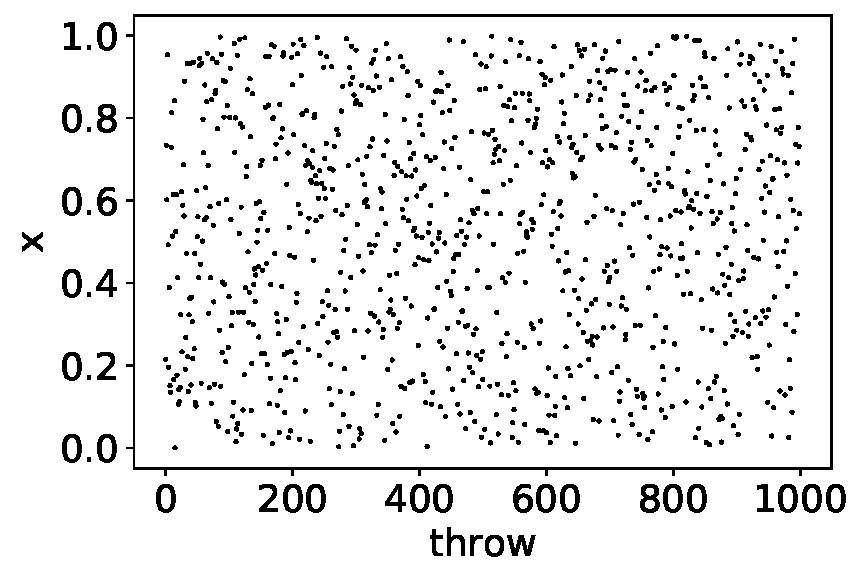
\includegraphics[height=0.22\textheight]{figs/monte_carlo/flat2d.pdf} &
  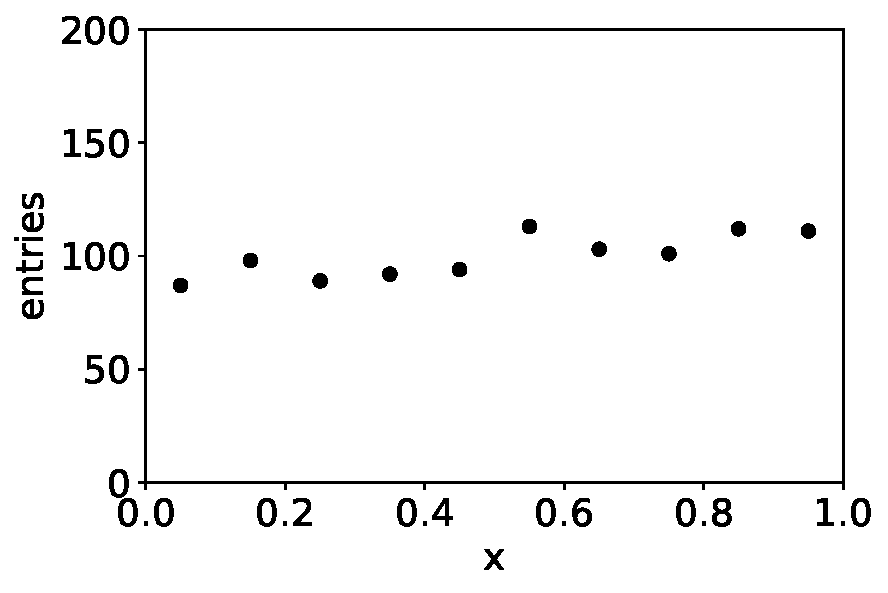
\includegraphics[height=0.22\textheight]{figs/monte_carlo/flathist.pdf} \\
  (a) & (b) \\
 \end{tabular}
\caption{The (a) $x$ value of uniform random throws versus throw number and (b) corresponding histogram. }
\label{fig:flathist}
\end{center}
\end{figure}

\noindent
How can we verify that our Park-Miller random number generator
produces uniform random numbers in the range 0 to 1?  The associated
PDF is just $p(x)=1$, which we know how to plot, but how can we
compare this function to a sequence of numbers like $[0.21, 0.85,
  0.33, ...]$?  An initial attempt might look like
Fig.~\ref{fig:flathist}a, where we have simply plotted the $x$ value
of each throw versus the number of the throw.  Unfortunately, this
plot isn't particularly helpful.  If we zoomed in, we could determine
from the plot the $x$ value associated with each throw.  This is
simply too much information.

For interpreting a list of values as a distribution, there is only one
tool of choice: the histogram.  To histogram our data, we divide the
entire range $[0,1]$ into smaller ranges called {\em bins}.  Let's
start with 10 bins as an example. In this case, the first bin covers
the range from 0 to 0.1, or more precisely, the half-open interval
$\left[0,0.1\right)$ which includes $0$ and $0.099$, but not $0.1$.
  The second bin would have range $\left[0.1,0.2\right)$, the third
    bin would have range $\left[0.2,0.3\right)$ and so on, up to the
      last bin which would cover $\left[0.9,1.0\right]$.  To {\em
        fill} a histogram, you count the number of values that fall
      within the range of each bin.  So in our example, the value
      $0.21$ would add one to the count for the third bin, which has
      range $\left[0.2,0.3\right)$.  After filling, the histogram
        consists of a count associated with each bin range.

Fig.~\ref{fig:flathist}b shows a histogram filled with 1000 random
throws drawn from a uniform random number generator.  While we can now
see the shape of the distribution, we still don't have quite enough
information to answer the question, is this flat?  It is certainly not
perfectly flat!

The first feature we will need to add to the plot is the inclusion of
{\em error bars} to indicate the statistical uncertainty in our
histogram values.  Error bars are conventionally drawn with a size
equal to the standard deviation of the measured value, $\sigma$.  Each
histogram contains a {\em count} $n$.  As we will see in lecture, this
count is drawn from a Poisson distribution, and our best estimate for
the standard deviation $\sigma$ associated with a count $n$ is simply
$\sqrt{n}$.  So when drawing a histogram, the uncertainty in each bin
is simply the square root of the histogram value.  That is the beauty of
Poisson statistics!  If we have a count, we know the statistical
uncertainty.

\begin{figure}[htbp]
 \begin{center}
  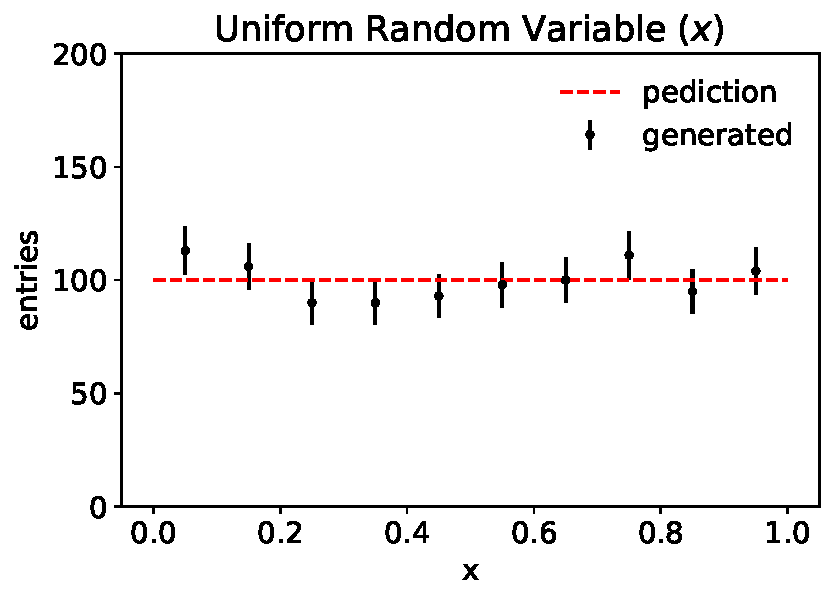
\includegraphics[width=0.50\textwidth]{figs/monte_carlo/fancyhist.pdf}
  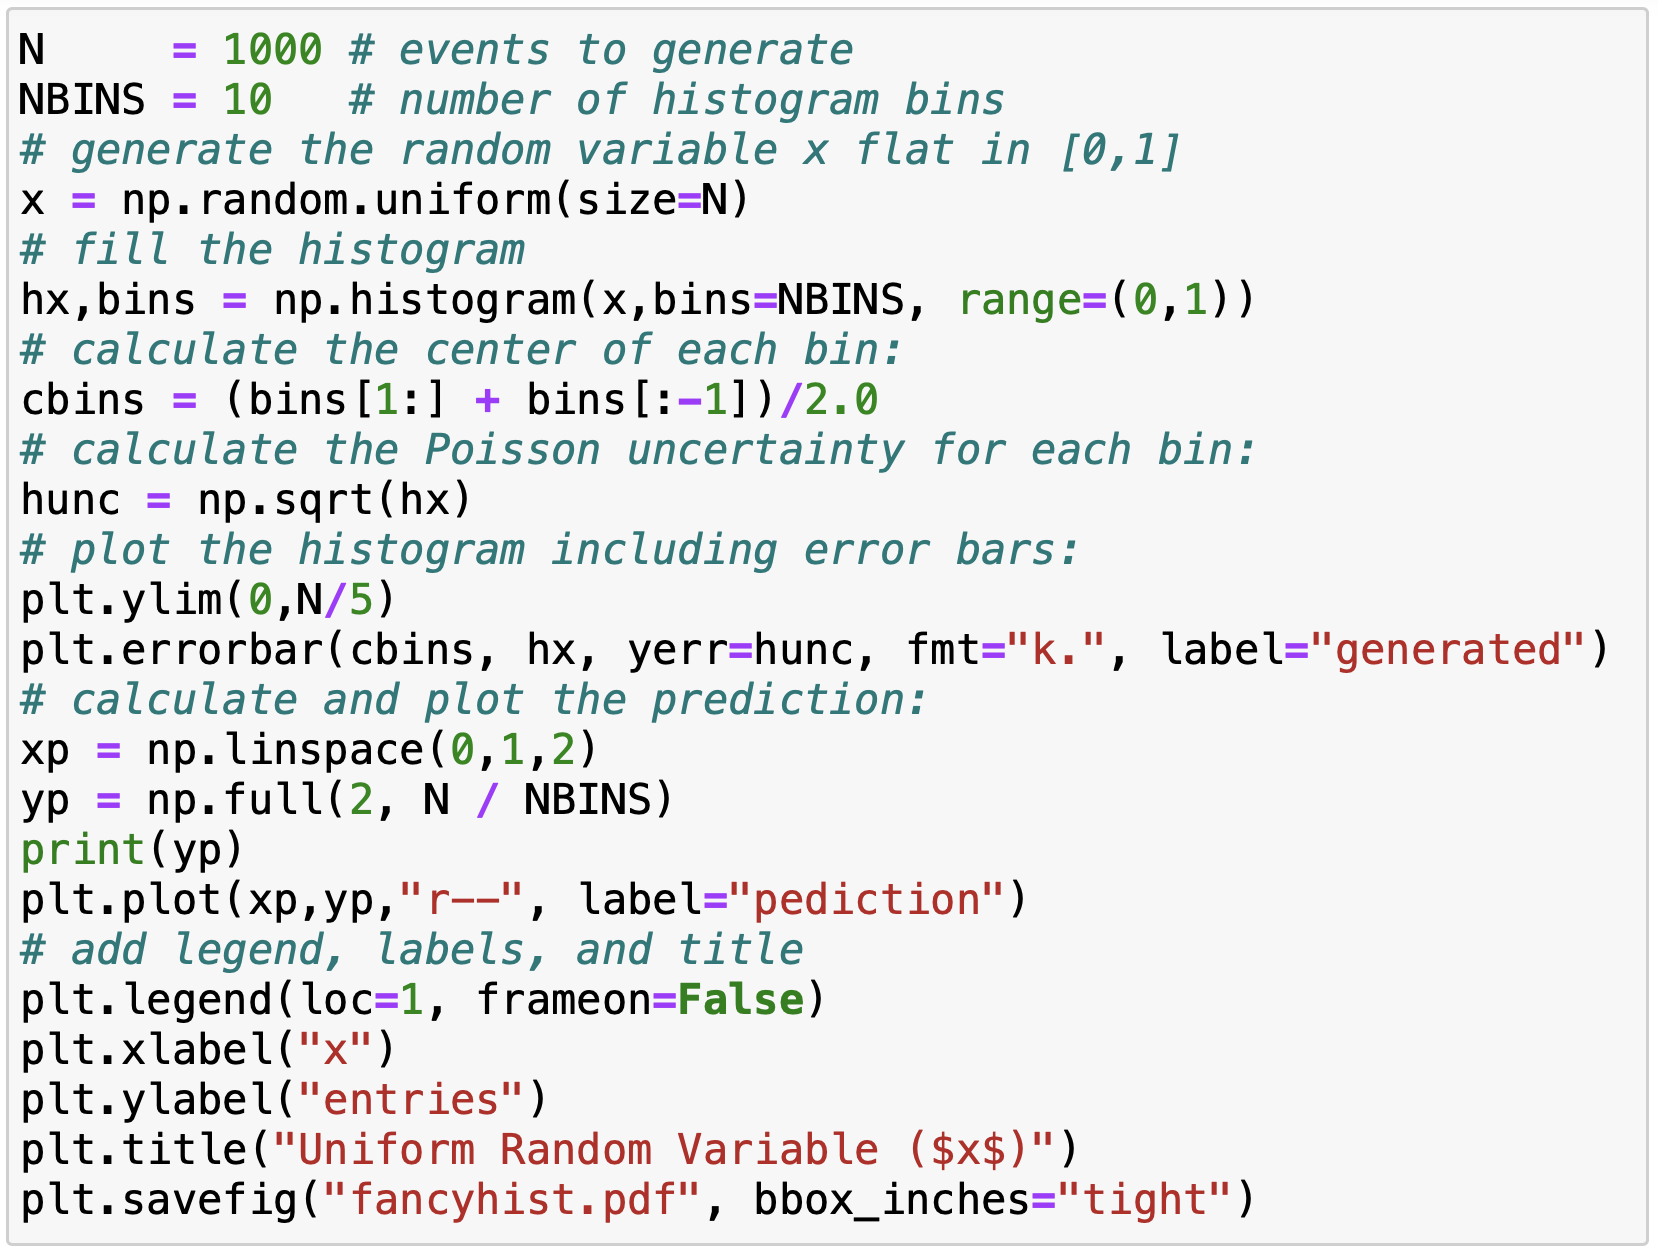
\includegraphics[width=0.75\textwidth]{figs/monte_carlo/fancyhist-code.png}
\caption{Histogram of data drawn from a flat distribution compared to prediction, with the code used to produce the plot.}
\label{fig:fancyhist}
\end{center}
\end{figure}

We'll also want to add the prediction to the plot, assuming a flat
distribution for the contents of each bin.  In this case, we generated
$N$ events and we have $N_{\rm BINS}$ histogram bins, which should
therefore each contain an equal share: $N / N_{\rm BINS}$.  The
resulting histogram, along with the code used to generate it, is shown
in Fig.~\ref{fig:fancyhist}.  With the prediction and errorbars
included in the plot, one can now see that these generated values are
indeed quite consistent with a flat prediction. All of the bins are
within nearly one-sigma. With this number of bins, it is not uncommon
to see a two-sigma descrepancy.

You will produce many histograms in this class, so you will need to
(eventually) understand every single line in this example code.  Take
the time to read through the documentation for the key functions like
{\tt np.histogram} and {\tt np.random.uniform}, available on the web
(see numpy.org or just search ``np.histrogram python'').  A big part
of learning to program effectively, is learning how to read and
understand software documentation correctly and efficiently.

There are a few important features to notice:
\begin{itemize}
 \item The $x$-values are contained in an {\tt np.array} filled with
   uniform random variables generated by calling the {\tt
     np.random.uniform} function.
 \item The function {\tt np.histogram} is used to calculate a histogram
   from these $x$ values.  The call requests {\tt NBINS=10} histogram
   bins, in range $[0,1]$.  Don't confuse the python tuple {\tt (0,1)}
   used to indicate this range as indicating an open interval... often
   the computing language differs significantly from math notation, as
   is the case here!
 \item The {\tt np.histogram} function returns two items we need:  a {\tt np.array} containing the count for each bin ({\tt hx}) and a {\tt np.array} of bin edges ({\tt bins})
 \item We want to plot the count over the center of each bin, not one of the edges, so we calculate the quantity {\tt cbins} which is an {\tt np.array} containing the center of each bin.  You'll use this trick a lot, so make sure you understand what it is doing!
 \item The uncertainty on each bin {\tt hunc} is calculated as the square root of the bin counts {\tt hx}.
 \item We use the somewhat poorly named {\tt np.errorbar} function to plot {\bf both} the histogram central value {\tt and} the errorbar in each bin.
 \item We draw the prediction as a straight line defined by two points defined by {\tt xp} and {\tt yp}.
\end{itemize}

\begin{plot} \end{plot}
Modify the example code to generate a histogram for uniform random
numbers generated from your Park-Miller sequence instead of ${\tt
  np.random.uniform}$.  Increase the number of events to {\tt
  N=10000}.  Increase the number of bins to {\tt NBINS=20}.  Does your
code appear to produce uniform random numbers?

To answer a question in your notebook, simply add a cell and answer the question as a comment (each line starting with {\tt \#}).

\section{Calculating the value of $\pi$}

\begin{figure}[htbp]
\begin{center}

\includegraphics[width=0.65\textwidth]{figs/monte_carlo/pitoss.jpg} 
\caption{Determining $\pi$ by throwing toothpicks.}
\label{fig:pitoss}
\end{center}
\end{figure}

\noindent
Hopefully 2021 will see the return of parties, so let's start by
examing a surefire way to be the life of the party: determining the
constant $\pi$ by throwing toothpicks!  The procedure is simple: you
cut a peice of paper to a width of four toothpicks, then draw two
vertical lines separated by the width of two tooth picks.  Take turns
tossing toothpicks, as in Fig.~\ref{fig:pitoss}.

From the geometry of the setup, it can be shown that the probability
that a toothpick which is entirely on the paper also crosses a line is
given by $1/\pi$.  Therefore, one can measure $\pi$ by counting the
total number of toothpicks that landed entirely on the page and
dividing by the number of those toothpicks that crossed a line.  This
is, in essence, the Monte Carlo method.

\begin{figure}[htbp]
\begin{center}
  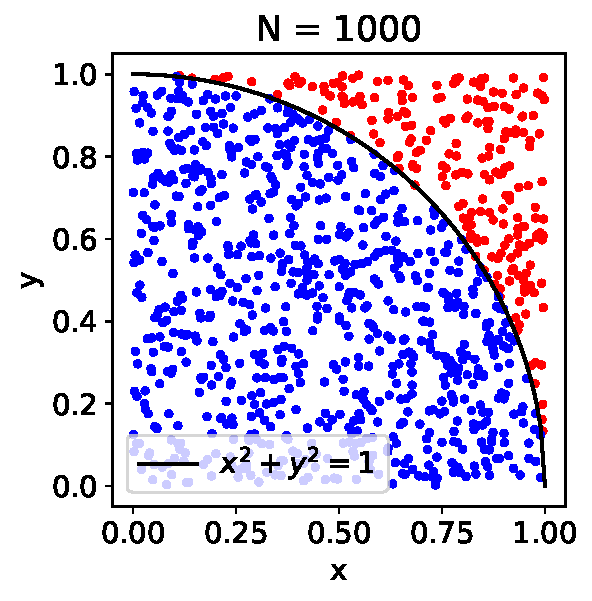
\includegraphics[width=0.50\textwidth]{figs/monte_carlo/pimc.pdf}
  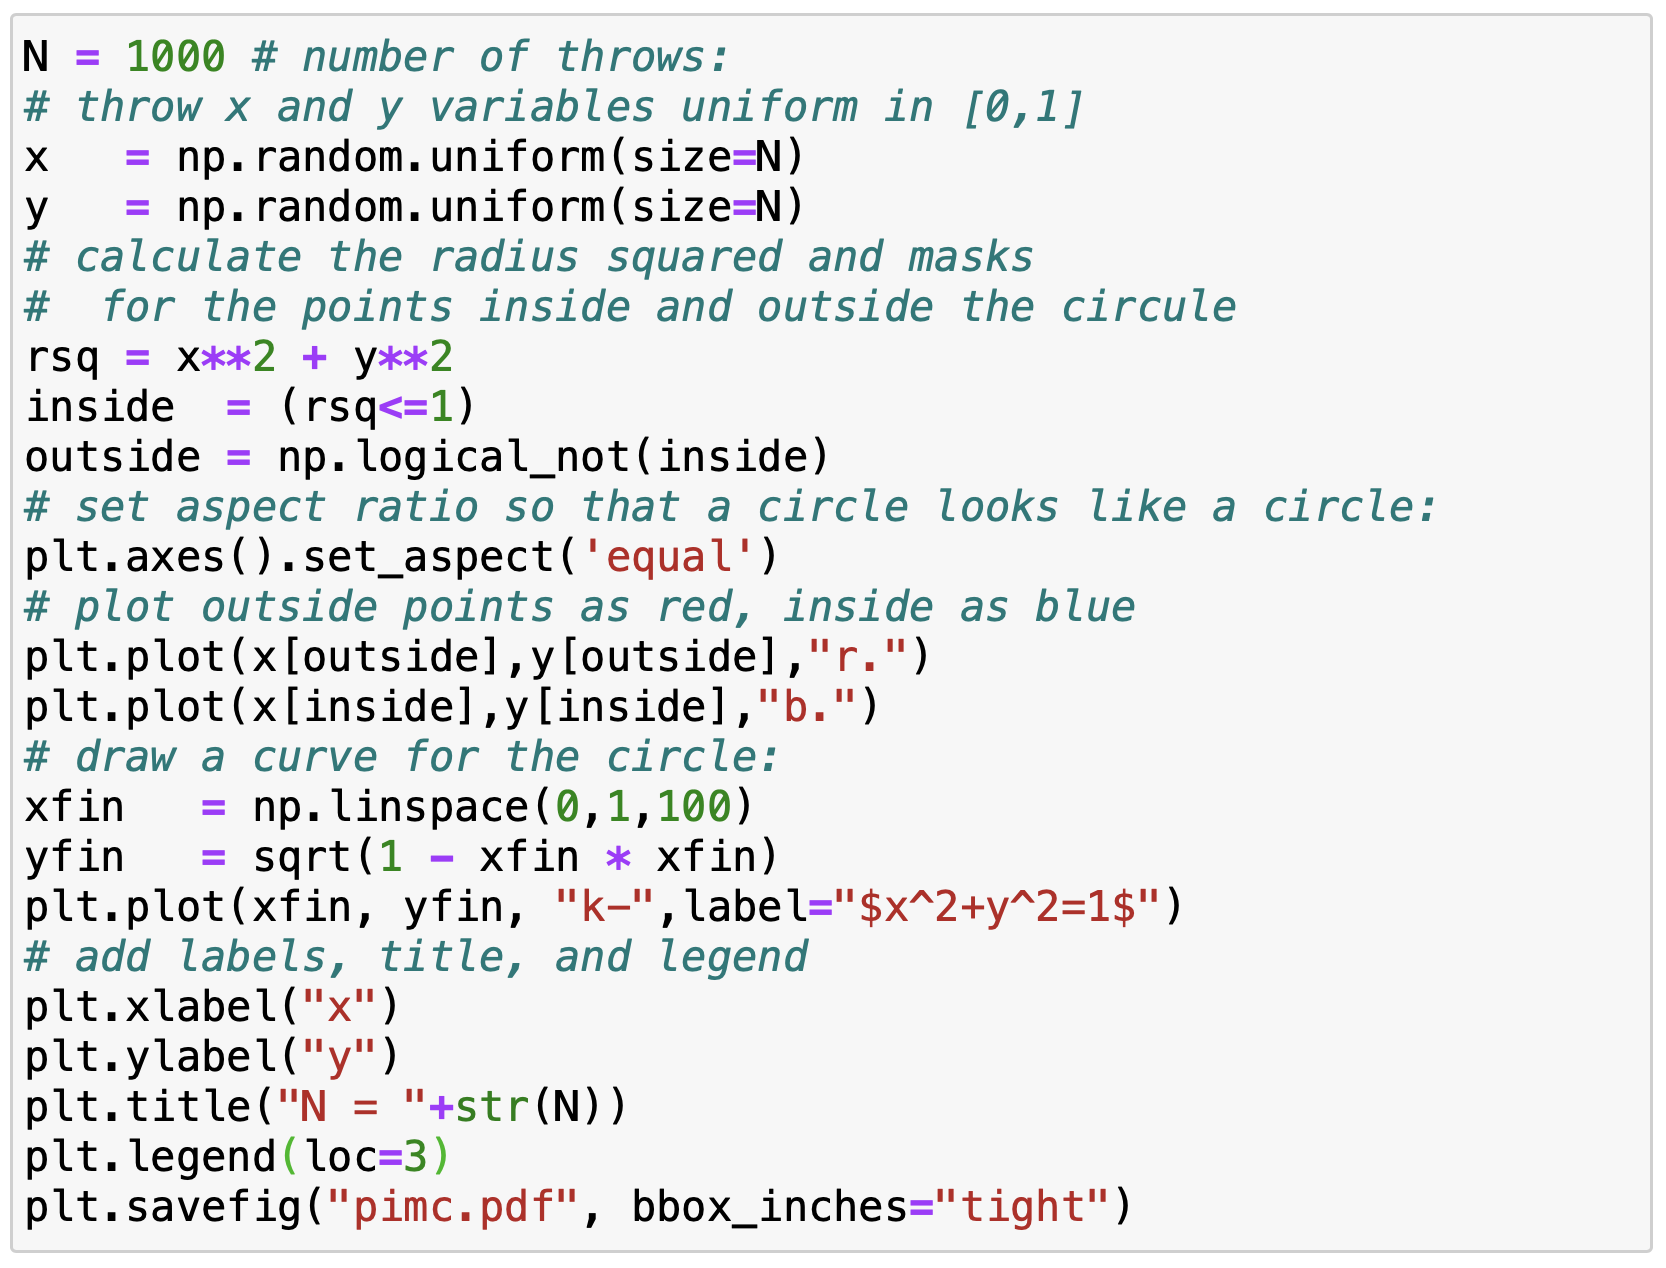
\includegraphics[width=0.75\textwidth]{figs/monte_carlo/pimc-code.png} 
\caption{Monte Carlo Determination $\pi$ .}
\label{fig:pimc}
\end{center}
\end{figure}

An easier Monte Carlo method to implement computationally is shown in
Fig.~\ref{fig:pimc} along with the code used to generate the plot.
The idea is to throw points uniformly in the unit square of area 1.
Much like in the toothpick example, the value of $\pi$ can be
determined by counting the number of generated points that also landed
within the unit circle.

The key features of the example code are:
\begin{itemize}
\item The $x$ and $y$ values are each contained in an {\tt np.array} filled with uniform random variables in $[0,1]$ by the {\tt np.random.uniform} function.
\item A mask {\tt inside} is created to indicate which points are inside the circle.  Recall that the mask is an {\tt np.array} of True or False values, with the same length as the $x$ and $y$ arrays.  For example {\tt x[inside]} is an np.array containing just the subset of {\tt x} which are inside the circle.  
\end{itemize}

\begin{plot} \end{plot}
Starting from the example code, determine the numerical value of $\pi$
using the Monte Carlo method.  The easiest way to obtain the count you
need is to apply the function {\tt np.sum} to an appropriate mask.
When counting a mask, each True is treated as a one, and each False is
treated as zero.  Work out the relationship between $\pi$ and the
fraction of events in the unit circle, and use your count to
numerically determine the value of $\pi$.  Increase the number of
generated events and confirm that your calculated value of $\pi$
approaches the known value.

\begin{plot} \end{plot}
This is an example of a binomial process, because points are either
inside or outside the circle. So we expect the number of events in the
circle to follow the binomial distribution with $\sigma^2 = n \epsilon
(1-\epsilon)$.  In this case, $n$ is the total number of generated
events and $\epsilon$ is the fraction that fall inside the unit
circle.  The statistical uncertainty on your measured value of $\pi$
works out to be:
\begin{displaymath}
\sigma_\pi = \sqrt{\frac{\pi \, (4-\pi)}{n}}
\end{displaymath}
where $n$ is the number of generated events.  Does your measured value
of $\pi$ agree with the known value within your statistical
uncertainty?

\section{Monte Carlo integration}

The Monte Carlo method can also be used to numerically integrate a
function.  Monte Carlo integration methods generally only outperform
deterministic methods when the number of dimensions is large, but we
can illustrate the method most easily in one dimension. In this
section, you'll use the Monte Carlo method to perform the integral:
\begin{displaymath}
  \int_0^\pi \sin^2 \theta \, d\theta
\end{displaymath}

To do so, you should make a copy of your solution from the previous section
and modify it in the following manner:
\begin{itemize}
 \item Instead of thowing $x$ in $[0,1]$, throw $\theta$ in $[0,\pi]$.  This means the area of the rectangle $A$ is now $\pi$ instead of 1.
 \item Count the number of throws that land below the integral $y < \sin^2 \theta$.
 \item Determine the area under the curve as the fraction of the throws under the curve times the total area of the rectangle $A$.
 \item The statistical uncertainty in this case is $\pi/(2\sqrt{n})$ where $n$ is the number of generated events.
\end{itemize}  

\begin{plot} \end{plot}
Use the Monte Carlo method to calculate the integral:
\begin{displaymath}
  \int_0^\pi \sin^2 \theta \, d\theta
\end{displaymath}
Make a plot similar to that of Fig.~\ref{fig:pimc} showing the thows
above the curve in red and below the curve in blue.  Calculate the
integral and statistical uncertainty and compare it to the value you obtain analytically.

\section{The Rejection method}

\begin{figure}[htbp]
\begin{center}
  \begin{tabular}{cc}
  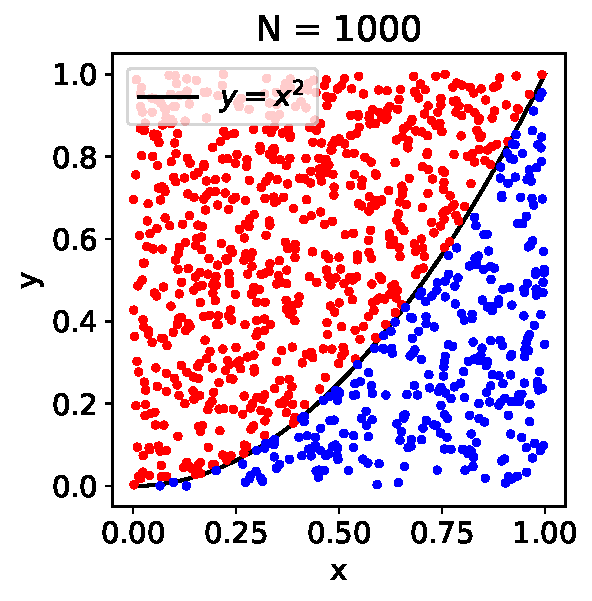
\includegraphics[height=0.30\textheight]{figs/monte_carlo/rejectmc.pdf} &
  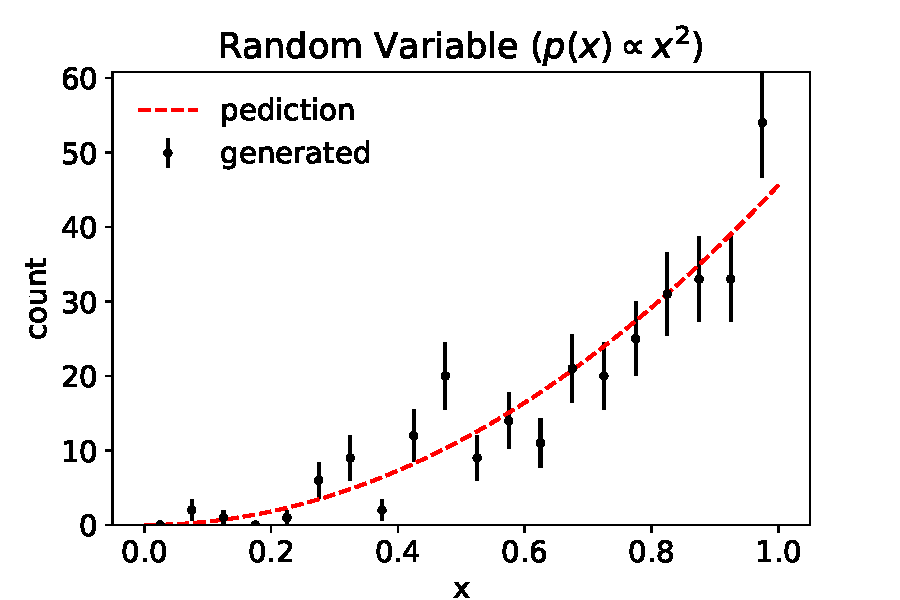
\includegraphics[height=0.30\textheight]{figs/monte_carlo/quadhist.pdf} \\
  (a) & (b) \\
 \end{tabular}
  \caption{Monte Carlo rejection method applied to $p(x) \propto
    x^2$. Uniformly generated points (a) are rejected (red) if they
    are above the PDF, and the $x$ values of points below the PDF
    (blue) are selected.  A histogram (b) of the selected $x$ values
    shows that they follow the PDF.}
  \label{fig:rejectmc}
\end{center}
\end{figure}

\noindent
We now know how to generate uniform random numbers, but suppose we
need a random variable thrown according to a non-uniform probability
distribution $p(x)$?  Fig.~\ref{fig:rejectmc} demonstrates one
approach, which closely follows the procedure for numerical
integration using the Monte Carlo technique.

The rejection method produces random variables in a range from 0 to $L$
according to any desired PDF $p(x)$.  Start by finding a value $Y$ which is at
least as large as the maximum value of $p(x)$ for $x$ in $[0,L]$.  Then:
\begin{itemize}
  \item Throw $x$ as a uniform random variable in range $[0, L]$.
  \item Throw $y$ as a uniform random variable in range $[0, Y]$.
  \item If $y > p(x)$ reject the $x$ value and start over, otherwise, use the $x$ value as one throw.
\end{itemize}
Repeat these steps as necessary until a sufficent number of $x$ values have been selected.

The rejection method works because the probability of an $x$ value
being selected is, by construction, proportional to $p(x)$.  Since the
$x$ values were initially chosen from a flat distribution, the
selected $x$ values will follow the $p(x)$ distribution.  You can
visualize this in Fig.~\ref{fig:rejectmc} which leaves very little
doubt that the $x$ values of the blue points will follow the PDF.
Notice that it isn't even necessary for $p(x)$ to be normalized for
this procedure to work: any function proportional to the PDF of interest will do.

To produce a smooth function such as the quadratic prediction of
Fig.~\ref{fig:rejectmc}b, make sure you use plenty of $x$ values
(around 100 at least), via {\tt np.arange} or {\tt np.linspace}, just
as you did in the Plotting lab.  When comparing a PDF to histogrammed
data (as you will do for the second plot below) you will need to
normalize it appropriately.  The number of throws we expect to find in
a bin with edges at $a$ and $b$ is given by
\begin{displaymath}
  N \cdot \int_a^b p(x) \, dx \; = N \cdot p(x^*) \cdot (b-a) 
\end{displaymath}
The integral is simply the probability that one throw ends up in the
range, which we scale by the total number of throws $N$.  The equality
holds for at least one $x^*$ in the range $[a,b]$ and $(b-a)$ is
simply the bin size.  Therefore, we can formulate a prediction from a
normalized PDF $p(x)$ to data from $N$ throws used to fill a histogram with
bin sizes $\Delta x$ as the smooth function resulting from:
\begin{displaymath}
N \cdot p(x) \cdot \Delta x
\end{displaymath}
This is a technique we will use over and over again, so make sure you
understand it!

\begin{plot} \end{plot}
Use the rejection method to generate random numbers in the region from [0,1] that follow a distribution $p(x) \propto x^2$.  You'll do the following:
\begin{itemize}
  \item Note that there is no need to normalize the PDF when using the rejection method, so use $p(x)=x^2$.
  \item In our $x$ range $[0,1]$, $p(x)$ has maximum value at $x=1$ so set $Y = p(1) = 1^2 = 1$. 
  \item Throw $x$ as a uniform random variable in the range $[0, 1]$.
  \item As $Y=1$, throw $y$ as a uniform random variable in range $[0, 1]$.
  \item If $y > x^2$ reject the $x$ value and try a new set of $x$ and $y$ values, otherwise, use the $x$ value as one throw.
\end{itemize}
Throw 1000 (unselected) $x$ values, and produce a plot like that of
Fig.~\ref{fig:rejectmc}a showing your selected points in blue, your
rejected points in red, and the selection function ($p(x) = x^2$).

\begin{samepage}
\begin{plot} \end{plot}
Increase the number of (unselected) $x$ values thrown to 10,000.
Count the number $N$ of selected $x$ values.  Generate a plot like that of
Fig.~\ref{fig:rejectmc}b comparing the distribution of your selected
$x$ values to the prediction, which in this case is given by:
\begin{displaymath}
N \cdot 3x^2 \cdot \Delta x
\end{displaymath}
Be careful to use the number of selected $x$ values for $N$, not the total thrown (10000) before rejection.
\end{samepage}

\section{The transformation method}

Suppose that you need to throw random variables according to an
exponential distribution $p(x) = \exp(-x)$.  This PDF is defined for
$[0,+\infty)$ and properly normalized across this range as you can verify:
\begin{displaymath}
  \int_0^{+\infty} \exp(-x) \, dx = 1
\end{displaymath}    
The first problem is that we can only generate uniform random
variables up to a finite value $L$, not $+\infty$.  But let's suppose we are
willing to work aound this by simply cutting off the PDF at some large
value, like say we won't produce values with $x>100$.

With this change, the rejection method will work in principle.  But it
still has a major shortcoming.  Since $p(x)$ has a maximum value of 1,
and $x$ ranges from 0 to 100, the rectangle we will be filling with
uniform random points has area 100.  But our PDF, even when
integrated to $+\infty$, only has area 1.  So less than one out of
every 100 points we throw will be selected.  Perhaps we can live with
this, but then what if we need to go out to $x=1000000$.  Now only one
out of every million points will be selected.  In many scenarios, the
rejection method becomes too computationally inefficient to be of any
practical value.

In these case, we can use the transformation method instead of the
rejection method.  The transformation method is premised on the fact
that for {\em any} normalized PDF, we must have
\begin{displaymath}
  p(x) \geq 0
\end{displaymath}
everywhere and
\begin{displaymath}
  \int_{-\infty}^{+\infty} p(x) \; dx = 1
\end{displaymath}
as long as we take care to set $p(x)=0$ outside our range for $x$.  It follows from these properties that for any value of $y$ in the range $[0,1]$ there is a unique largest $x$ value for which:
\begin{equation} \label{eqn:mctransform}
  \int_{-\infty}^{x} p(x) \; dx = y
\end{equation}
From the fundamental theorem of calculus, we see that:
\begin{displaymath}
  dy = p(x) \, dx
\end{displaymath}
If the variables $y$ are drawn from a uniform distribution with PDF $q(y)=1$, then we see that:
\begin{displaymath}
 \int_{y_1}^{y_2} q(y) \, dy = \int_{x_1}^{x_2}p(x) \, dx.
\end{displaymath}
for $x_i$ and $y_i$ related by Eqn.~\ref{eqn:mctransform}.  This shows
that while $y$ is a uniform random variable ($q(y)=1$), the
corresponding $x$ values will distributed according to the desired PDF
$p(x)$.

That provides the mathematical justification for the transformation
method, which starts by finding the inverse function $f^{-1}(y)$ for:
\begin{displaymath}
  y = f(x) = \int_{-\infty}^{x} p(x) \, dx
\end{displaymath}
Then the procedure is:
\begin{itemize}  
 \item Throw $y$ as a uniform random variable in $[0,1]$.
 \item Find $x = f^{-1}(y)$
\end{itemize}
The $x$ values determined in this way will be drawn from the $p(x)$ distribution.  

There is an intuitive explanation for why this works.  The $y$ value is
essentially a fraction of the probability integrated by the PDF.  In a
region of $x$ where $p(x)$ is relatively large, the integral is
changing rapidly and so a large range of $y$ values map to this region
of $x$-values.  In a region of $x$ where $p(x)$ is relatively small,
the integral is not changing rapidly and so a small range of $y$
values map to this region of $x$-values.

Let's see how this applies to our exponential function.  In this case we calculate:
\begin{displaymath}
y = f(x) = \int_0^x \exp(-x) \, dx = 1 - \exp(-x)
\end{displaymath}  
which we invert to find:
\begin{displaymath}
x = - \ln(1-y)
\end{displaymath}  
To determine values of the random variable $x$, we follow this procedure:
\begin{itemize}
 \item Throw a $y$ value flat in [0,1]
 \item Caculate $x = -\ln(1-y)$
\end{itemize}
Repeat to produce as many $x$ values as needed.  Notice that this
procedure gives one usable $x$ value for every random throw.

\begin{plot} \end{plot}
Use the transformation method as described to generate 10,000 values
of a random variable thrown from an exponential function.  Produce a
plot like that of of Fig.~\ref{fig:rejectmc}b comparing the
distribution of your generated events to the prediction for $p(x) =
\exp(-x)$.  Remember to properly normalize your prediction based on
the bin size and number of events thrown.

\newpage
\section{Particle diffusion}

\begin{figure}[htbp]
\begin{center}
  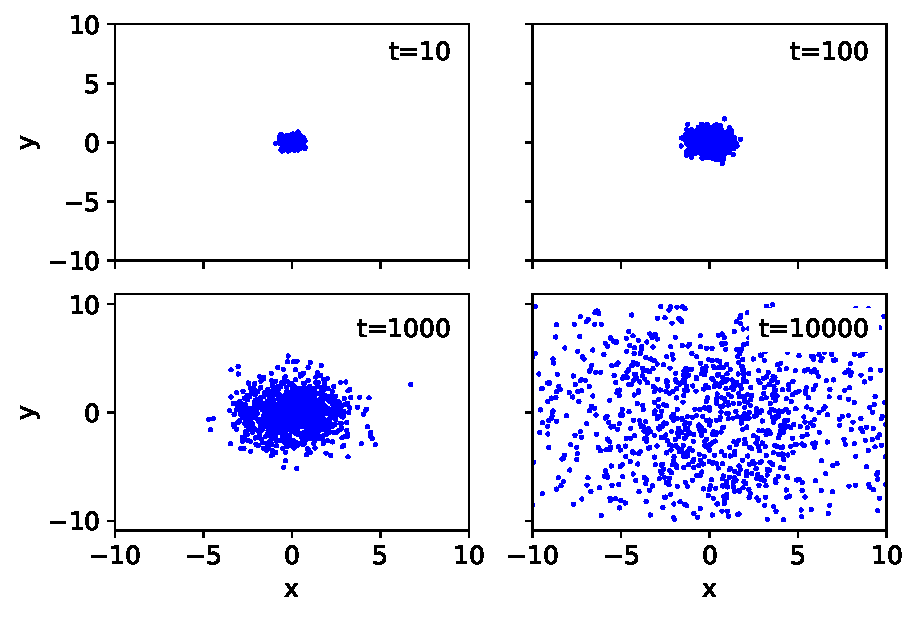
\includegraphics[width=0.80\textwidth]{figs/monte_carlo/diffusion.pdf}
  \caption{Simulation of the diffusion of a drop of particles at four different times.}
\label{fig:diffusion}
\end{center}
\end{figure}

\begin{figure}[htbp]
 \begin{center}
  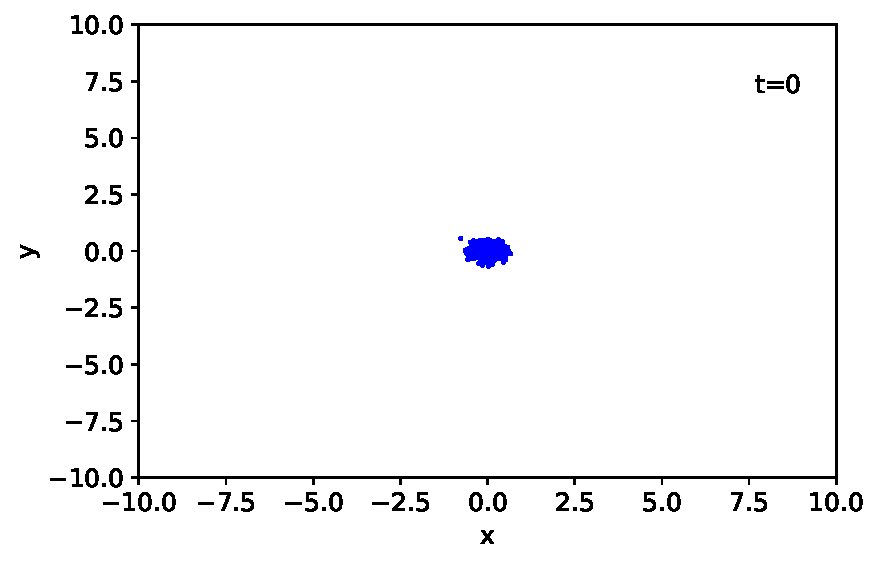
\includegraphics[width=0.50\textwidth]{figs/monte_carlo/diffstart.pdf}
  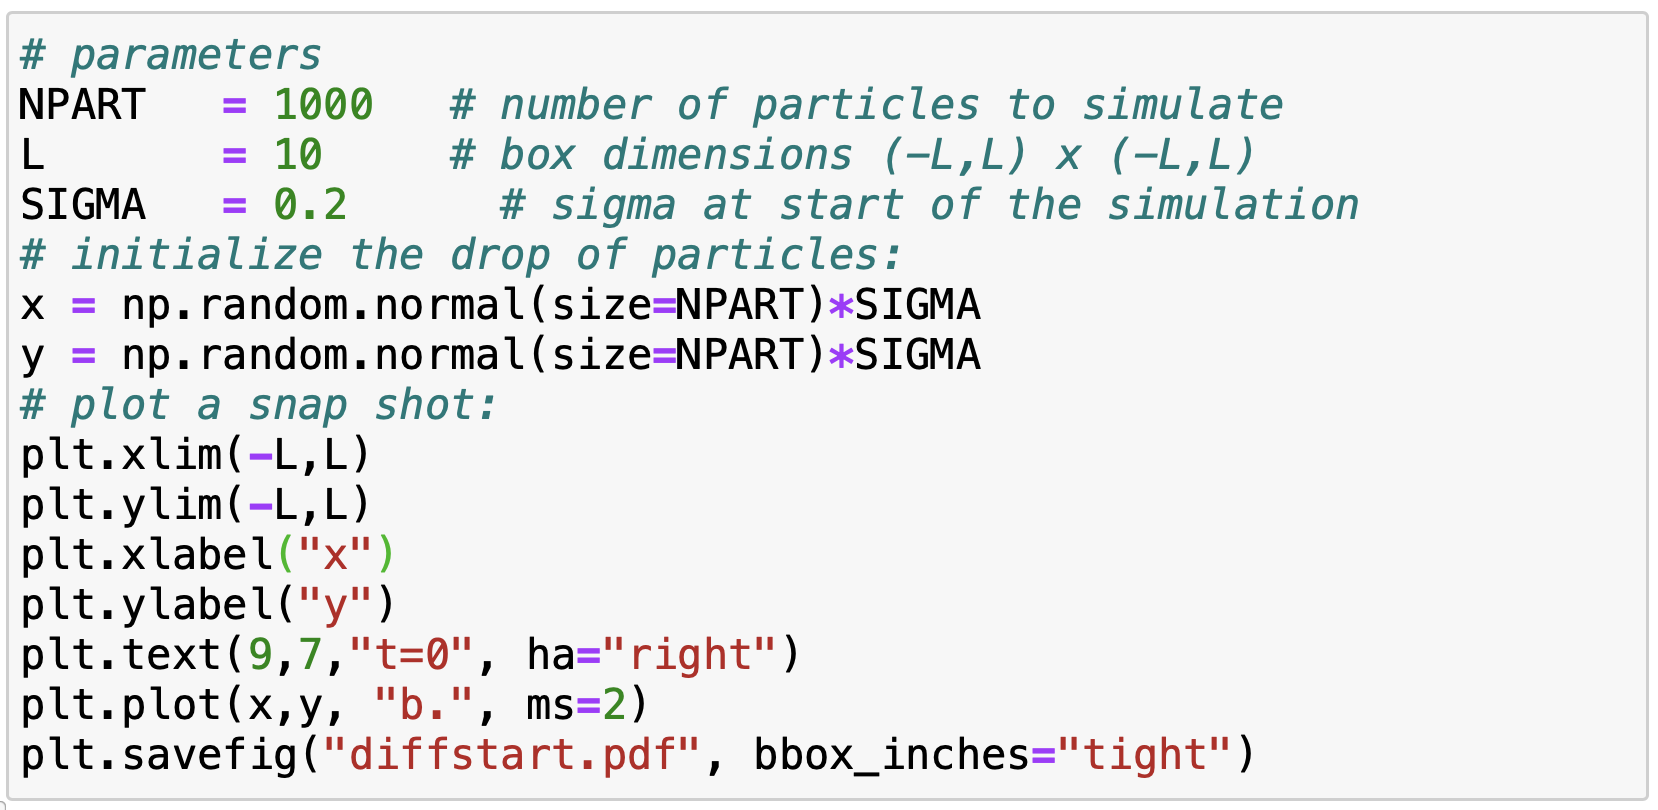
\includegraphics[width=0.75\textwidth]{figs/monte_carlo/diffstart-code.png}
  \caption{Snapshot of the simulation at the start, along with the code used to produce it.}
\label{fig:diffstart}
\end{center}
\end{figure}


\noindent
In this section, we will model the diffusion of a drop of particles in
a medium, as in Fig.~\ref{fig:diffusion}, shown as snapshots at four
different times.  The starting point for the simulation, at $t=0$ is
shown in Fig.~\ref{fig:diffstart} along with the code used to produce
it.  The entire state of the system is contained in the arrays {\tt x}
and {\tt y} which contain the $x$ and $y$ positions of each particle.

The diffusion process is modeled by a random walk. During each update
(for one time step) the $x$ and $y$ values of each particle should be
randomly increased or decreased by an amount {\tt STEP=0.2} Any
particles that would leave the boundaries of the region $[-L,L]$ as a
result should be moved back into the region.  The numpy functions 
{\tt np.random.choice} and {\tt np.clip} are useful here.

Despite the symmetry of the random walk, the system clearly evolves by
diffusing outward over time.  This can be seen as a consequence of the
second law of thermodynamics.  Calculating the entropy from the
microscopic state of continuous particles is a bit tricky.  The
approach we will use is based on the Gibb's entropy.  We divide the
area into cells, and determine the fraction of the particles $f_i$ in
each cell $i$.  We calculate the entropy as:
\begin{displaymath}
  S = \sum_i f_i \ln f_i
\end{displaymath}
A python function which calculates the entropy in this manner:
\begin{tt}
\begin{verbatim}
from scipy import stats  
def entropy(x,y,l,sbins):
    h,xbins,ybins=np.histogram2d(x,y,bins=sbins,range=[[-l,l],[-l,l]])
    return stats.entropy(h.flatten())
\end{verbatim}
\end{tt}
The function takes as input parameters the position arrays {\tt x} and
{\tt y}, the boundary distance {\tt l} (set it to {\tt L} and the
number of bins in each dimension {\tt sbins} (set it to 20).  The
function returns the entropy of the current state of the system
described by {\tt x} and {\tt y}.

\begin{plot} \end{plot}
Starting from the example code, implement a random walk to model the
diffusion process, and plot four snap shops showing the evolution of
the system.

\begin{plot} \end{plot}
Calculate and record the entropy of the system as it evolves, and plot
the entropy as a function of time.

